%
% The first command in your LaTeX source must be the \documentclass command.
\documentclass[sigplan]{acmart}

%
% defining the \BibTeX command - from Oren Patashnik's original BibTeX documentation.
\def\BibTeX{{\rm B\kern-.05em{\sc i\kern-.025em b}\kern-.08emT\kern-.1667em\lower.7ex\hbox{E}\kern-.125emX}}

\copyrightyear{2019}
\acmYear{2019}

\acmConference[]{}{}{}
\acmBooktitle{}
\acmPrice{}
\acmDOI{}
\acmISBN{}
\usepackage{indentfirst}
\usepackage{amsthm}
\usepackage{algorithm}
\usepackage{algpseudocode}

\newtheorem{myDef}{Definition}
\newtheorem{myTheo}{Theorem}

\renewcommand{\algorithmicensure}{\textbf{Class }}

\begin{document}
\title{Minimum Bounding Bicone: a new Minimum Bounding Box System for Trajectory Data}
\author{Liu Yinpei}
\email{lyp_bobi@yahoo.com}
\affiliation{%
  \institution{Shanghai Jiaotong University}
}
\begin{abstract}
In the widely used Minimun Bounding Box(MBB) system, if we want to express a moving object in a given time period, we have to form a 3-dimension rectangle that bound it, namely $[x_1,x_2] \times [y_1,y_2] \times [t_1,t_2]$. And when doing different kinds of query on the trajectories, we actually first use message of their MBBs to do some pruning to avoid the full scan of the database and the complex computation of the exact distance between trajectories. In this paper we propose a new method called Minimum Bounding Bicone (to make difference with Minimum Bounding Box, we abbreviate this as MBBC), which we would show to be a more precise description of the original trajectory points. And we designed a index structure named $R^2$-Tree, which could fully utilize the MBBCs to achieve better pruning power than R-Tree.
\end{abstract}

\maketitle

\section{Basic Observations and Hypotheses}
The index structure of spatial data is somehow matured now, as index structures like R-Tree, k-d Tree, space-filling curves, their variants, and other index structure have shown their efficiency on different realms in application. However, when comes to trajectory data, we find that these index structure can be further grained to become faster using the additional information and insight of real data. For trajectory data, we have some basic observations that is widely accepted: \\
\indent 1. Moving objects have only limited velocity, and the distance of a pair of adjacent points in one trajectory is hardly bounded according to the time difference of the points.\\
\indent 2. Enormous trajectory data is being produced every day, which naturally raised the necessity to use distributed databases and analysis tools.\\
\indent 3. The calculation of exact trajectory distance requires complex computation, so avoiding the exact calculation by pruning is very important.\\
\indent 4. The data are generally inserted in their time order, and updates to the past data is rarely needed.\\
\par
So there are some basic assumptions.\\
\indent 1. Most moving objects we are handling share a common acceptable speed bounds, like 30km/h for walking people, 200km/h for cars, 70km/h for ships. When handling spatio-temporal databases consists of two or more kinds of moving objects, build different indexes for different kinds is generally a good idea.\\
\indent 2. Although we don't assume the trajectory data to be stored in a distributed environment like HDFS, we would implement the algorithm in a distributed environment to achieve better scalability, which generally load a larger part of the data in a single I/O action. (For example, 64MB per block in HDFS instead of 8KB per page in Postgre SQL.) Note that the implementation on a non-distributed environment lead to no reduction of the pruning power of the index. \\
\indent 3. We have to do calculation on the trajectories instead of the points in the trajectories, so the real computation cost of the queries is polynomially higher than queries on the points.\par

Studies on trajectories have proposed the inefficiency of Minimum Bounding Boxes for a long time \cite{pfoser2000novel}, while good substitution to it are never provided to our knowledge. In this article, we would propose Minimum Bounding Bicone as a new bounding system for trajectory data. This system come from the basic idea that if we use the speed information, we could represent a uniform rectilinear motion a lot better than a MBB. And the trajectory of an objects in a short time period tend to be similar to a uniform rectilinear motion.\par


\section{Queries Supported}
We would like to support two basic kind of trajectory queries, namely range query and kNN query. Both of the query have multiple variants and different variants may require computing costs with polynomial level difference, so we would first give our definition of the query. \par
\begin{myDef}
  (ST-point) A Spatio-temporal point(abbreviate as ST-point) is a 3-tuple (x,y,t). The x and y stand for the location of the point, and the t stand for the time that the location is recorded.
\end{myDef}
\begin{myDef}
  (Trajectory) A trajectory is a list of ST-points sorted by their time value in ascendant order, namely

     $$[(x_1,y_1,t_1),(x_2,y_2,t_2),...,(x_n,y_n,t_n)], $$
     $$t_1 \leqq t_2 \leqq t_3 \leqq ... \leqq t_n .$$

   The trajectory is the sampled points of the real trajectory, which is in the form of the function
   $$T^{real}: t \Rightarrow (x,y), t\in [t_1,t_n].$$
   Notice that we assume we know exactly the starting and ending time of the real trajectory, namely $t_1$ and $t_n$.\\
   For the points are generally sampled in a given rate in the real world, we could assume that the differences $t_2-t_1, t_3-t_2, ... , t_n- t_(n-1)$ are nearly equal, although we don't require this property in the rest of the paper.
\end{myDef}
\begin{myDef}
  (Integral Distance) Given two trajectories $$T_a=[(x_{a1},y_{a1},t_{a1}), (x_{a2},y_{a2},t_{a2}), ..., (x_{am},y_{am},t_{am})]$$ and $$T_b=(x_{b1},x_{b1},t_{b1}), (x_{b2}, y_{b2}, t_{b2}), ..., (x_{bn}, y_{bn}, t_{bn}),$$ we define their Integral Distance as below:\\
  Denote $\hat{t}=\hat{t_a}\bigcup\hat{t_b}=\{t_{a1}, t_{a2}, ..., t_{am}\}\bigcup \{t_{b1}, t_{b2}, ..., t_{bn}\}$, and $\check{t}=[t_1, t_2, ..., t_l]$ as the $\hat{t}$ sorted by its ascendant order. And for $t \in \hat{t}$ define
  $$T_a'(t)=\left\{
             \begin{array}{lr}
             T_a(t), t \in \hat{t_a} \\
             T_a(t_{ak})+ (T_a(t_{a(k+1)})-T_a(t_{ak}))* \frac{t-t_{ak}}{t_{a(k+1)}-t_{ak}}, \\
             \indent  t \in [t_{a1}, t_{am}], t_{ak}<t<t_{a(k+1)} \\
             T_a(t_{a1}), t \in [t_{b1},t_{bn}] \setminus [t_{a1},t_{am}], t< t_{a1} \\
             T_a(t_{am}), t \in [t_{b1},t_{bn}] \setminus [t_{a1},t_{am}], t< t_{am}
             \end{array}
    \right.$$
  and $T_b'(t)$ similarly. Then the Integral Distance is
  $$
  \begin{aligned}
  d(&T_a,T_b)=\\
  &\sum_{i \in \{1, 2, ..., l-1\}} \frac{1}{2} (T_a'(t_i)-T_b'(t_i)+T_a'(t_{i+1})-T_b'(t_{i+1}))\\
  &\indent\indent\indent\indent\indent\indent\indent\indent\indent\indent*(t_{i+1}-t_i).
  \end{aligned}.
  $$
  This is a natural extension of the real Integral Distance
  $$\int_{t_1}^{t_l}(T_{a}^{real}-T_{b}^{real})dt.$$
\end{myDef}
\begin{myDef}
  (Range Query)Given a query box $$[x_1,x_2] \times [y_1,y_2] \times [t_1,t_2],$$return all the trajectories that "intersect", which means having at least one point inside, this box.
\end{myDef}
\begin{myDef}
  (kNN Query)Given a trajectory which not necessarily contained in the database, and find the trajectories which have the k smallest Integral distance to the given trajectory in the database, which may contain itself.
\end{myDef}

\section{Caculation of MBBC}
First we define a function which is at the core of this paper.
\begin{myDef}
  (Possible Area) Denote $\mathcal{C}$ as the full spatial space, which is invariant over time. Given a spatial area $\mathcal{A}$(which could degenerate into a point) and a time stamp $t_0$, we define the function $Possible\_Area()$ which calculate the Possible\_Area position at a given time $t$ if the object could at most move at a velocity $v$.
  $$
  Possible\_Area(t;\mathcal{A},t_0,v) = \{A+v|t-t_0|*\vec{n} \big| ||\vec{n}|| \leq 1\}.
  $$
\end{myDef}
\begin{myDef}
  (Possible Cone) We further define the function to calculate all the Possible\_Area points as Possible\_Cone(), which could be further divide extend to $Possible\_Cone^+$ and $Possible\_Cone^-$ as tow nappes of the double cone.
  $$
  \begin{aligned}
  Possible\_&Cone(\mathcal{A},t_0,v)=\\
  &\{Possible\_Area(t;\mathcal{A},t_0,v)\times t\}\\
  Possible\_&Cone^+(\mathcal{A},t_0,v)=\\
  &\{Possible\_Area(t;\mathcal{A},t_0,v)\times t \big| t\geq t_0\}\\
  Possible\_&Cone^-(\mathcal{A},t_0,v)=\\
  &\{Possible\_Area(t;\mathcal{A},t_0,v)\times t \big| t\leq t_0\}
  \end{aligned}
  $$
\end{myDef}
\begin{myDef}
(MBBC)Given a trajectory $$T=[(x_1,y_1,t_1), (x_2,y_2,t_2), ..., (x_n,y_n,t_n)],$$with the maximum speed v, the Minimum Bounding Bicone of it is
$$
\begin{aligned}
MBBC(T;v)=Possible\_Cone^+((x_1,y_1),t_1,v)\\
\bigcap Possible\_Cone^-((x_n,y_n),t_n,v),
\end{aligned}
$$
which is a bicone. As we can see, the intervening points contributes nothing to the MBBC after the maximum speed is given, so we call this type of MBBC a MBBC of points. %We could expression it by the 3-tuple $$((x_1,y_1,t_1),(x_n,y_n,t_n),v)$$. For the storage cost of the index is relatively small, we could also storage the MBB expressed as $$MBB=(MBBx_{min},MBBx_{max},MBBy_{min},MBBy_{max})$$ with the MBBC to enforce the pruning power. So we store a 4-tuple $((x_1,y_1,t_1),(x_n,y_n,t_n),v,MBB)$ to express a MBBC for a trajecory.
\par
Similarly we define MBBC of two area laid at starting and ending time, expressed as $(\mathcal{A},t_1),(\mathcal{B},t_n)$ to be
$$
\begin{aligned}
MBBC(\mathcal{A},\mathcal{B};t_1,t_n,v)=Possible\_Cone^+(\mathcal{A},t_1,v)\\
\bigcap Possible\_Cone^-(\mathcal{B},t_n,v),
\end{aligned}
$$
which shape would be like two truncated cones, so for convenience we still call it MBBC. \par
We call a MBBC with its $\mathcal{A}$ and $\mathcal{B}$ both rectangles, which may degenerate into a line segment or a point, as a regular MBBC.
Due to the strategy of building the index tree, the $\mathcal{A} and \mathcal{B}$ of each MBBC mentioned in this paper would be rectangles. So in the rest of paper we assume every MBBC is regular without extra explanation.
\end{myDef}

%Although we could define a MBBC by such parameters, in implementation, the MBBC should also store the intersection point of the projection of the MBBC on x-t surface and y-t surface to avoid calculation on pruning, which will be discussed in Chapter \ref{sec:query}. We call the four intersection points as nodes, where xnodes stand for those on the y-t suface, and ynodes the ones on x-t surface. The pseudo code of MBBC and MBB would be like \ref{alg:class}.

\begin{algorithm}[ht]
%\floatname{algorithm}{CLASS}
%\newcommand{\algorithmname}{CLASS}
%\renewcommand{\thealgorithm}{}
\caption{Class Statement} \label{alg:class}



\begin{algorithmic}[0]
\Ensure Point
    \State dimension:Int
    \State x:Double
    \State y:Double
    \State t:Double

\Ensure MBB
    \State dimension:Int
    \State low:Point //this Point stores the lower value of x,y and t for this MBB
    \State high:Point //this Point stores the higher value of x,y and t for this MBB

\Ensure MBBC
    \State A:MBB //start area, dimension=2
    \State B:MBB //end area, dimension=2
    \State maxspeed:Double //the maxspeed of this layer
    \State mbb:MBB //the MBB when dimension=3

\Ensure pointMBBC \textbf{extends} MBBC
    \Function{x}{}
    \State \textbf{return} A.x1
    \EndFunction
    \Function{y}{}
    \State \textbf{return} A.y1
    \EndFunction
\end{algorithmic}
\end{algorithm}

The shape of the MBBC of a trajectory would like Figure \ref{fig:matlab}. Notice that the volume of a cone is 1/3 of the volume of the cylinder, which would obviously result in stronger pruning power.\\
\begin{figure}[ht]
  \centering
  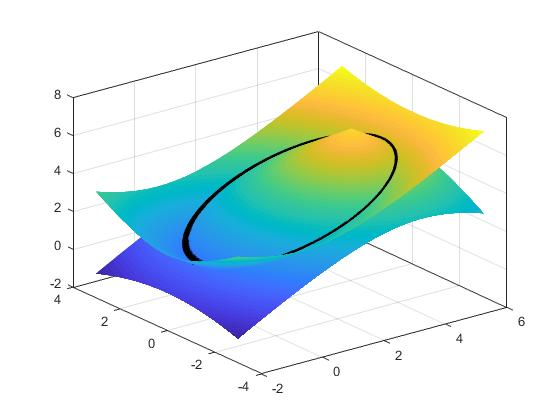
\includegraphics[width=\linewidth]{matlab.jpg}
  \caption{A MBBC of points,Plotted by MATLAB, with speed 1, start point (0,0,0), and end point (4,0,5)}
  \Description{matlab bicone}
  \label{fig:matlab}
\end{figure}


\section{Building Index on MBBCs}
MBBC is a tight expression to the raw trajectories, but the use of the maximum velocity leads to some problems when we want to combine multiple MBBCs to construct a RTree-like structure, as the slope of different MBBCs are different. To overcome this problem, we would combine multiple MBBC as they all moving at the maximum speed at this time period.\par
\subsection{building the index}
We choose to build a $B^+$-Tree or a Hash table on the time axis, and for each time period(which is a leaf of the $B^+$-Tree or a value of the Hash table), we would build a RTree-like index structure called $R^2$-Tree. The square means that it use the range informations both at the start time and at the end time. We are doing this for four reasons.\\
\indent The first reason is the inefficiency of RTree and its variants on 3 or higher dimensions. This basically comes from the fact that the ratio of volume of the bounding boxes in comparison with the real volume grows exponentially with the increase of dimension.\\
\indent The second reason is that the query on the trajectories generally only involves trajectories in a given time period instead of using time information as a measurement of the relation between trajectories.\\
\indent The third reason is that things can move forth and back in spatial axes, but can only move forth in time axes. Using $B+$-Tree or Hash table could utilize this knowledge better.\\
\indent And the last reason is that scholars have agreed on the necessity of cutting long trajectories into small segments to avoid their MBBs to grow too large. We would also use this method to avoid producing large MBBCs, and this method basically corresponds to the division of time axis.\par

We suggest two ways to build the first level of index upon time axis. The first one is to divide the time into segments of a given length, for example, one hour. Then we can access the $R^2$-Tree of the given time period by Hash Table. But this method may lead to data imbalance, for example, the car trajectories during the day is more than the trajectories during the night. The imbalance of data would not only lead to the imbalance of the whole tree, but also the imbalance of pruning power, that is, if there are a lot of trajectories in a given time period, we would want the time period to be smaller or the MBBCs would be overlapped with others frequently and make it hard to pruning using spatial information. So we suggest a second way, which is to build a $B^+$-Tree where each leaf node shares almost the same number of trajectory points. For general data, this method would result in longer querying time, but for skewed data, this method may produce better result.\par

In each time period, if the time period is $[t_1,t_n]$, we would build the so called $R^2$-Tree, which by structure is a binary tree, in a simple divide and conquer manner. At start, we have a root node which record all the trajectories in $$MBBC(\mathcal{C},\mathcal{C};t_1,t_n,v).$$ Then we would either do a "start division" or a "end division", the process would be similar to the construction of k-d Tree.\par

For start division, we pick an area $\mathcal{A}$ and calculate the $$\mathcal{B}=MBB(Possible\_Area(t;\mathcal{A},t_1,v)).$$
Then we calculate $$\mathcal{B'}=MBB(Possible\_Area(t;\mathcal{C} \setminus \mathcal{A},t_1,v)),$$
which is the area that an object can reach if it start in $\mathcal{C}\setminus \mathcal{A}$. So the left node of the root is the trajectories in $$MBBC(\mathcal{A},\mathcal{B};t_1,t_n,v),$$ and right node is the trajectories in $$MBBC(\mathcal{C}\setminus \mathcal{A},\mathcal{B'};t_1,t_n,v).$$ The end division is just the same except we first pick an area containing ending points, and calculate back the Possible\_Area starting position.\par

The area selection is just like the k-d Tree, where we first select an axis, and for the axis, we select the median point and divide the plain into two parts which would divide the data into two sets containing equal number of trajectories. For there are two spatial dimensions, we have four division strategies, namely start/end division along x/y axis.\par

Due to the division strategy, the starting and ending area of MBBCs would always be rectangle, which we mentioned before. This makes calculation of checking intersection easier.

In every step, we would choose the one from the four strategies whose child nodes contains least volume. So although the MBBCs are overlapping each other inevitably, we could still try to minimize the number of MBBCs to overlap with a query box, which intuitively would lead to better pruning result. If two or more of the strategies have the same child nodes volume, we would randomly pick one.\par
% We would use them in circle on different level of the tree, for example, start division along x-axis for the first level of the tree, end division along x-axis on the second, start division along y-axis for the third level, end divisions along y-axis for the fourth level, and continue with the descendent levels.

The division strategy should stop when every node is small enough, which should roughly have contains the data that can be read out by one I/O action. (e.g. 8KB for Postgre SQL and 64MB for databases based on HDFS)

\subsection{MBB and real maxspeed Construction}
Although we use MBBCs to express the set of trajectories, we can still use MBB to enforce the pruning power. And we could label each MBBC with it's real max speed instead of the global one to further empower the pruning method. These two information of a tree node can be calculated directly by using the information of its child nodes. So by a bottom-up method applied to the tree after the division phase, we could append the information of exact MBB of the whole trajectory, the exact MBB of the starting area, the exact MBB of the ending area, and the exact max speed to each tree node to enhance the pruning power. \par
So every tree node of the index would contain two MBBCs, one for inserting new data so that every trajectory could be insert into a leaf node, the other for the exact message for the pruning.\par
Note that the MBBs and real maxspeed may have to update when new data is inserted or old data is modified.\par


\subsection{Building a two level Index}
The modern distributed system tend to do I/O action in bulk mode, in other word, read a big bulk of data, like 64MB in HDFS, for one I/O action, instead of the classical mode of reading a page of 8KB or something like that each time. So now we don't have to consider the I/O cost at the leaf-side of the index tree too much. Instead, we just use the first level of index to find the related partition of the data, and load all these partition into memory for further processing. And the second liar of the index, which is referred as "local index" in multiple papers, was build in memory for further pruning and retrieval. \par
To build a global and local index doesn't have much difference to the construction of one level of index. The only difference is that the global index part contains the part of global index contains the $B^+$-Tree or Hash Table to index the divisions of time period, while the part of local index only contains the $R^2$-Tree.\par
When building global index, the tree-node division procedure would end when each partition is small enough, which generally should be decide by the platform, for example, 64MB or 128MB for HDFS. If data update is needed, we would suggest to use only 40\% to 80\% of the maximum capacity of a leaf node in case their would be more data to insert. As stated earlier, we suppose that we don't have to change the past data a lot, so this structure would generally be good enough. \par
%The local index is just like the Global index, the only difference is that when use the maximum speed of this partition(which is recorded as "actual maximum speed" in global index) to build the $R^2$-Tree. At the leaf nodes, they don't directly contain the data, but still the reference to the data and the MBBC, so we could do the most specific pruning.



\section{Querying using Index} \label{sec:query}
As we mainly support range and KNN query, the most important questions we have to answer when using the index are these two:\\
\indent 1. How to decide whether a MBBC intersects with a MBB with the least computation cost?\\
\indent 2. How to calculate the minimum and maximum distance between two MBBCs with low computation cost?\par
Intuitively, these calculations seems to be time costing. That is what people generally argues about for an oriented bounding box system, which is widely discussed in the realm of collision detection.(They call the MBB along axes as AABB method, and not along axes as OBB method.) But these calculation of MBBC could be tolerable using the property of the bicones.\par

\subsection{Doing Range Query}

Given a query box MBB, we first have to prune out most of really irrelevant data using most simple calculation, so we first calculate
$$\mathcal{A} = MBB(Possible\_Area(t_0;[x1,x2] \times [y1,y2], t_2, maxspeed)$$
and
$$\mathcal{B} = MBB(Possible\_Area(t_n;[x_1,x_2] \times [y_1,y_2], t_1, maxspeed).$$
Where the maxspeed is the theoretical one instead of the exact one. Using this, all the MBBCs that the starting area don't intersect with $\mathcal{A}$ or ending area don't intersects with $\mathcal{B}$ would be pruned easily. If we have the exact MBB message, we can instead use the message of MBBs to do this round of pruning by checking whether the MBB intersects with the query box. \par
After the first level of pruning, we can use some more costy algorithm for the most of data is already pruned out. So we would start to check whether the MBBC actually intersects with the MBB.\par
A good property of bicone is that when looking from any direction which is perpendicular to t-axis, the shape of the bicone is a parallelogram with the same slope (which is the value of maximum speed v). We could easily proof that if a MBBC intersects with a MBB, then their projections on x-t plane, y-t plane and x-y plane also intersect. We would use this property for the second stage of pruning, named Projection Pruning. \par

Using the fact that the absolute value of the slope of each edge of the parallelogram is the same, we could transform the condition stated above into some simple comparison, as shown in Algorithm \ref{alg:proprune}. Although there could be more pruning, we should consider that the exact computation of collision is unacceptable, and some false positive is acceptable.
\begin{algorithm}
\caption{ProjectionPruning} \label{alg:proprune}
\begin{algorithmic}[1]
\Function{ProjectionPruning}{bc:MBBC, box:MBB}
    \State maxspeed:Double = bc.maxspeed
    \State t0:Double = box.low.t-bc.A.t
    \State t1:Double = box.high.t-bc.A.t
    \State t:Double = bc.B.t-bc.A.t
    \State d:Double = maxspeed*t
    \State a:Double
    \State b:Double
    \State //check the y-t surface projection
    \If{bc.A.x+bc.B.x>box.high.x+box.low.x}
        \State a=bc.A.x-box.high.x
        \State b=bc.B.x-box.high.x
    \Else
        \State a=box.low.x-bc.A.x
        \State b=box.low.x-bc.B.x
    \EndIf
    \If{a+b>d or a*t>d*t1 or b*t>d*(t-t0)}
        \State \textbf{return} false //pruning
    \EndIf
    \State //check the x-t surface projection
    \If{bc.A.y+bc.B.y>box.high.y+box.low.y}
        \State a=bc.A.y-box.high.y
        \State b=bc.B.y-box.high.y
    \Else
        \State a=box.low.y-bc.A.y
        \State b=box.low.y-bc.B.y
    \EndIf
    \If{a+b>d or a*t>d*t1 or b*t>d*(t-t0)}
        \State \textbf{return} false //pruning
    \EndIf
    \State //check the x-y surface projection
    \If{$d^2+(box.A.x-box.B.x)^2+(box.A.y-box.B.y)^2>(2*box.x-box.A.x-box.B.x)^2+(2*box.y-box.A.y-box.B.y)^2$}
            \State \textbf{continue}
    \EndIf
    \If{(bc.A.x-bc.B.x)(bc.A.y-bc.B.y)>=0}
        \If{not \Call{InEllipse}{bc,Point(box.low.x,box.high.y)} \textbf{and} not \Call{InEllipse}{bc,Point(box.high.x,box.low.y)}}
            \State \textbf{return} false
        \EndIf
    \Else
        \If{not \Call{InEllipse}{bc,Point(box.low.x,box.low.y)} \textbf{and} not \Call{InEllipse}{bc,Point(box.high.x,box.high.y)}}
            \State \textbf{return} false
        \EndIf
    \EndIf
    \State \textbf{return} true
\EndFunction
\Function{InEllipse}{bc:MBBC,point:Point}
    \If{$(bc.A.x-point.x)^2+(bc.A.y-point.y)^2+(bc.B.x-point.x)^2+(bc.B.y-point.y)^2>d^2/4+(bc.A.x-bc.B.x)^2+(bc.A.y-bc.B.y)^2$}
        \State \textbf{return} false
    \EndIf
\EndFunction
\end{algorithmic}
\end{algorithm}

\subsection{Doing KNN Query}
How to do KNN query in a R-tree like structure have been studied widely.\cite{nnq95} And the most popular method is to use the MINDIST(the minimum possible distance given the information of the MBBs) and MINMAXDIST(the guranteed value that the exact minimum distance must smaller or equal to).\par
However, the exact calculation of MINDIST on trajectories requires too much calculation, while the calculation of MINMAXDIST can only be evaluated as MAXDIST(the maximum possible distance given the information of MBBs) as there are multiple points and the MBB yield too little information.\par
By using the MBBC method, we could yield tighter bounds to MINDIST and MAXDIST, make it a lot tolerable to calculate. \par
The strategy we use is rather simple, we first calculate the distance of two MBBCs at the starting and ending points, and combine them with max speed to yield a most pessimistic and optimistic distance as MINDIST and MAXDIST. The pseudo code is in Algorithm \ref{alg:minmax}.\par
The Algorithm would just like the KNN algorithm on the R-Tree. When we are given a distance d and a trajectory traj, we don't have to run the code of calculating MINDIST and MAXDIST on every node in the tree. Instead, we can only concern the nodes that distance of the starting time plus distance of the ending time is lesser to $3* maxspeed* t + 2*d/t$, which could be search quickly through the $R^2$-Tree
\begin{algorithm}
\caption{MINDIST and MAXDIST} \label{alg:minmax}
\begin{algorithmic}[1]
\Function{MINANDMAX}{bc1:MBBC, bc2:MBBC}
    \State maxspeed:Double = max(bc1.maxspeed,bc2.maxspeed)
    \State min:Double
    \State max:Double
    \State d1:Double = $(bc1.A.x+bc2.A.x)^2+(bc1.A.y+bc2.A.y)^2$
    \State d2:Double = $(bc1.B.x+bc2.B.x)^2+(bc1.B.y+bc2.B.y)^2$
    \State m1:Double = $(bc1.A.x+bc1.B.x)^2+(bc1.A.y+bc1.B.y)^2$
    \State m2:Double = $(bc2.A.x+bc2.B.x)^2+(bc2.A.y+bc2.B.y)^2$
    \If{$d1<(2*maxspeed*t)^2$ \textbf{and} $d2<(2*maxspeed*t)^2$} //then they could meet
        \State min = (d1*d1+d2*d2)/maxspeed/4
    \Else
        \State t = bc1.B.t-bc1.A.t
        \State min = (sqrt(d1)+sqrt(d2))*t-maxspeed*t*t/2-2*(d1+d2)/maxspeed
    \EndIf
    \State max = (sqrt(d1)+sqrt(d2))*t + maxspeed*t*t/2+ 2*(d1+d2)/maxspeed
    \State \textbf{return} (min,max)
\EndFunction
\Function{MINANDMAX}{traj:List[Point], bc:MBBC}
    \State maxspeed:Double = bc.maxspeed
    \State ts:Double = traj[0].t
    \State te:Double = traj[-1].t //-1 means the last one
    \State d1 = $sqrt((traj[0].x+bc.A.x)^2+(traj[0].y+bc.A.y)^2)$
    \State d2 = $sqrt((traj[-1].x+bc.B.x)^2+(traj[-1].y+bc.B.y)^2)$
    \State summin:Double = d1* (traj[1].t- traj[0].t) + d2* (traj[-1].t-traj[-2].t)
    \State summax:Double = d1* (traj[1].t- traj[0].t) + d2* (traj[-1].t-traj[-2].t)
    \For{i = 1,2,3,...len(traj)-2}
        \State summin += max(d1+(traj[i].t-ts)*maxspeed, d2+ (te-traj[i].t)*maxspeed,0)* (traj[i+1].t-traj[i-1].t)
        \State summax += max(d1+(traj[i].t+ts)*maxspeed, d2+ (te+traj[i].t)*maxspeed)* (traj[i+1].t-traj[i-1].t)
    \EndFor
    \State \textbf{return} (summin/2,summax/2)
\EndFunction
\end{algorithmic}
\end{algorithm}

\section{Implementation on Spark}
In this section we will show how to implement the two-level of global index and one level of local index in a widely used distributed platform, namely Apache Spark.\par
In Spark, there are naturally two levels of storage. The first level is RDD, which is open to the users, and stand for the data to be analysed. The second level is partition. Each RDD is divided into many partitions which is about 64MB each to store in HDFS, and when Spark have to analysis the data in a RDD, it just read the related partition to reduce I/O cost. The partition is generally transparent to users. The RDD is a structure optimized for analysis, so the insertion and deletion cost are very high.\par
Recent studies have proposed a widely used method called two-level index, which refers to a structure that use a global index to manage different partitions, and use a local index to handle the data inside a single partition. \par
Instead of just adopting the two-level index structure, we extend it into a three-level index using the property of time axis. This method would help us to append new data into the data set, modified the past data, and update index more easily, which cater to the real application better.\par
At the top level, instead of represent the whole data as one RDD, we use a combination of RDDs to store data. Each RDD stands for a leaf node of the $B^+$-Tree or a hash value of Hash Map in the time axis of global index. So when modifying data, we don't have to reconstruct the whole data, instead, we could just reconstruct the related RDD./par
In addition, since the data volume would be very large, we also designed a memory scheduling algorithm which take use of the spatial and temporal information, called spatial-LRU, to reduce the I/O cost.\par

This part is incomplete.


\bibliographystyle{ACM-Reference-Format}
\bibliography{sample-base}


\end{document}












